
\documentclass[answers]{exam}
%%%%%%%%%%%%%%%%%%%%%%%%%%%%%%%%%%%%%%%%%%%%%%%%%%%%%%%%%%%%%%%%%%%%%%%%%%%%%%%%%%%%%%%%%%%%%%%%%%%%%%%%%%%%%%%%%%%%%%%%%%%%%%%%%%%%%%%%%%%%%%%%%%%%%%%%%%%%%%%%%%%%%%%%%%%%%%%%%%%%%%%%%%%%%%%%%%%%%%%%%%%%%%%%%%%%%%%%%%%%%%%%%%%%%%%%%%%%%%%%%%%%%%%%%%%%
\usepackage{amssymb}
\usepackage{amsmath}
\usepackage{pdfpages}
\usepackage{marvosym}
\usepackage{hyperref}
\usepackage{enumitem}
\usepackage{tikz}
\usepackage{graphicx}
\usepackage{float}
\usepackage{soul}
\usepackage{multirow}

\setcounter{MaxMatrixCols}{10}
%TCIDATA{OutputFilter=LATEX.DLL}
%TCIDATA{Version=5.00.0.2552}
%TCIDATA{<META NAME="SaveForMode" CONTENT="1">}
%TCIDATA{LastRevised=Wednesday, February 16, 2011 02:52:30}
%TCIDATA{<META NAME="GraphicsSave" CONTENT="32">}
%TCIDATA{Language=American English}

\topmargin=-1.8cm \textheight=23.8cm \oddsidemargin=-0.3cm
\evensidemargin=-0.5cm \textwidth=17.1cm
\newtheorem{ass}{Assumption}
\newtheorem{prop}{Proposition}
\newtheorem{thm}{Theorem}
\newtheorem{lem}{Lemma}
\newtheorem{conj}{Conjecture}

\begin{document}


\thispagestyle{empty}\baselineskip1.2\baselineskip\

\noindent \textbf{Econ 140\newline
Summer 2022 \newline
Instructor: Fernando Hoces de la Guardia \newline
GSIs: Elena Stacy \& Yige Wang
}

\vskip2ex

\noindent \textbf{Midterm Exam 2}

\vskip3ex

\noindent \textbf{Tuesday July 26, 2022}

\vskip9ex


%\vspace{2.5in}

\noindent Student Name:

\vskip5ex

\noindent Student ID Number:
\vskip9ex
\noindent \textbf{Exam Instructions:}


\begin{itemize}
\item \textbf{You have 80 minutes to answer this exam} 

\item \textbf{This exams has a total of 80 points (suggesting the length of time to spent in each question). Each question indicates the number of points, and indicates a maximum length for its answer} 

\item \textbf{Most questions ask for short answers (from a couple of words, to one or two sentence maximum)} 
\item \textbf{Explanation in black or blue ink is recommended as these often scan the best.} 
\item \textbf{You must submit your solutions using the exam packet provided.} 
\item \textbf{Do not write your solutions on pages that say ``Do not write solutions on this page"}. Answers written on these pages will not be graded. You may use these pages as scratch paper.
\item \textbf{When time is called, STOP} writing, immediately \textbf{CLOSE} your exam packet and hold it up until it is collected.
\item \textbf{Show your work}. Credit will only be awarded on the basis of what is written on the exam.
\item \textbf{Sign the academic honesty pledge}. Cheating will be punished.
\end{itemize}

\newpage


\vskip10ex

\noindent \textbf{Affirm the academic honesty pledge below}. For those writing on a non-printed copy, please just write ``Academic Honesty Pledge as on exam'', and sign your name. \\\textbf{\underline{If you do not affirm this pledge, your exam will be marked invalid.}}


\vskip12ex

\noindent \textbf{0. ACADEMIC HONESTY PLEDGE }

\noindent I confirm that I have abided by all academic honesty rules for UC Berkeley and Economics 140. I confirm that I did not see this exam before my official exam start time. I confirm that I have not shared and will not share this exam with anyone else. I confirm that I haven't copied from anybody else's exam.

\vskip5ex

Signature: \hrulefill

\vskip5ex
\vspace{5cm}

Formula for the SE of $\widehat \beta$ in a bi-variate regression: 

$$
SE(\widehat \beta) = \frac{\sigma_{e}}{\sqrt{n}} \times \frac{1}{\sigma_X}
$$

 \begin{figure}[H]
    \centering
    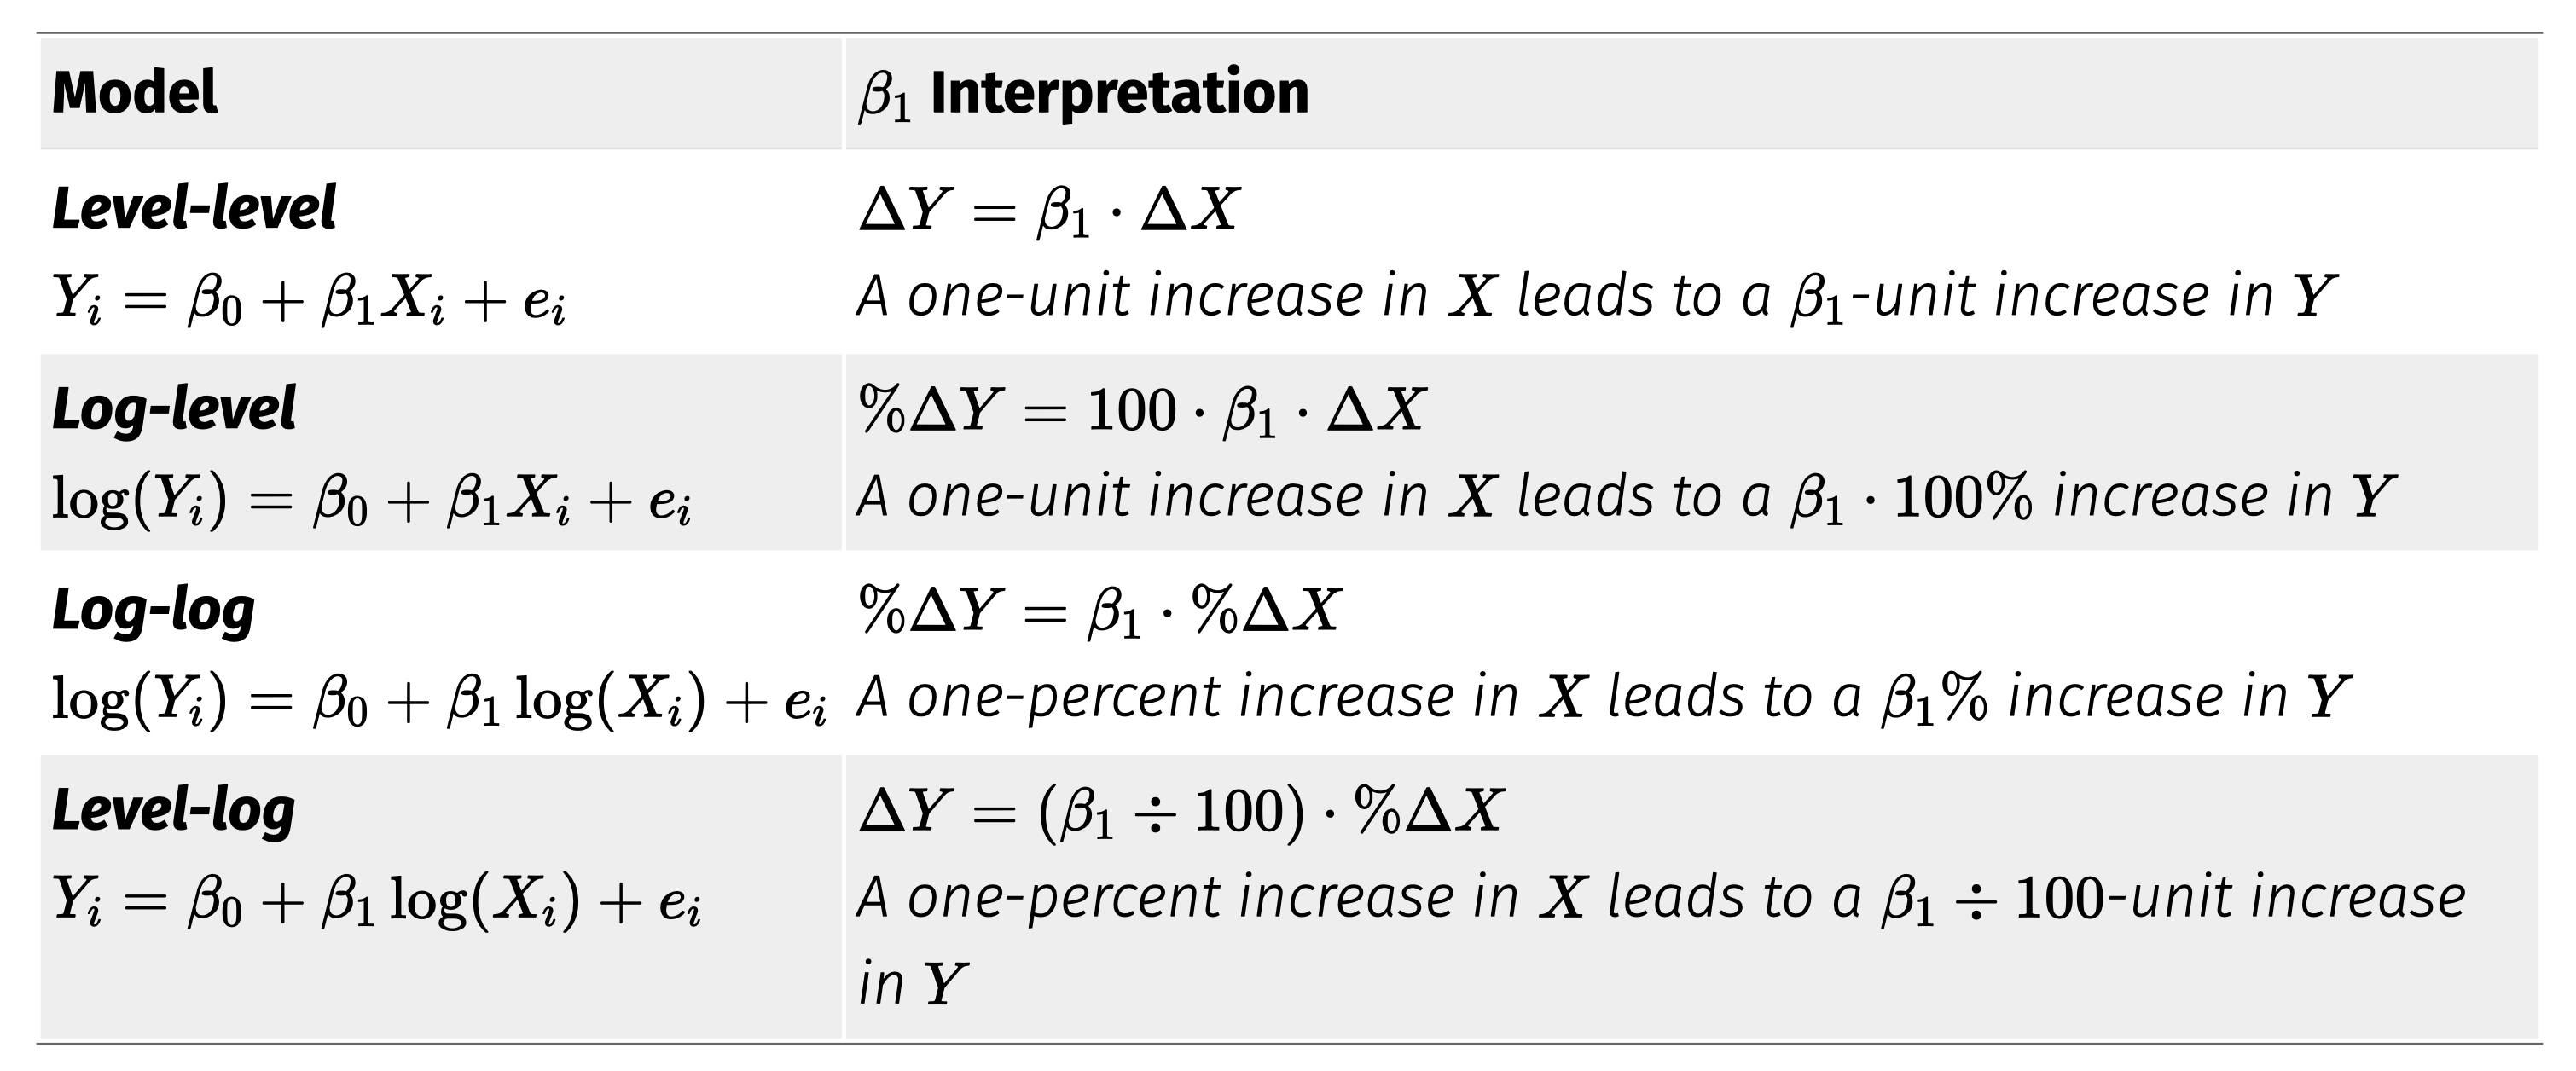
\includegraphics[width=6in]{Figures/midterm2_ref.png}
    %\caption{}
    \label{}
\end{figure}

\newpage

%\noindent \textbf{1. Short Questions (15 points, 3 points per question.)}

\vskip1ex

\begin{enumerate}
\item For the Oregon Health Plan Experiment (OHP), describe in one sentence, one of the two key policy questions that the experiment shed light on (considered only as relevant information from Ch1).[2pts, 1 sentence]
\vspace{3cm}
\begin{solution}
Two possible solutions:
\begin{itemize}
    \item OHP studies studies the effect of receiving an offer of free health insurance, among a vulnerable population in Oregon, on their (mental and physical) health. 
    \item OHP studies studies the effect of receiving an offer of free health insurance, among a vulnerable population in Oregon, on their financial security (or financial health). 
\end{itemize}

\end{solution}


\item RCTs are simple in logic, but difficult in logistics. In the RAND Health Insurance Experiment (HIE) discussed in class, the original design had a total of 14 treatments, but when preforming the analysis, this 14 were groups into 4 broader categories. The researchers did this to address which of the following concepts discussed in class [2pts]
 \begin{enumerate}[label=\alph*)]
    \item Increase sample size to address the fundamental problem of identification
    \item Reduce the logistical burden of tracking individuals over 14 different insurance services. 
    \item Increase sample size so the estimated coefficients can be approximated by well-known distributions.
    \item Reduce variation in the error term. 
   \end{enumerate}
\begin{solution}
C
\end{solution}

\item When conducting a hypothesis test in a regression analysis our main goal is [2pts]: 
\begin{enumerate}[label=\alph*)]
    \item Check if the estimated coefficient is consistent with some population parameter
    \item Check if an observed statistic is large in magnitude
    \item Check if the t-statistic is larger than 2 or smaller than -2
    \item Check if the population coefficient is consistent with a range around our estimated parameter.
 \end{enumerate}
\begin{solution}
A
\end{solution}

\item Explain in one or two sentences how assigning an intervention on \textbf{the basis of who needs it most would NOT solve} the selection bias problem (an example of need-based assignment would be to assign health insurance to the people that have the worst health, or are poorer, first). [3pts, 2 sentences]
\begin{solution}
"All else equal" is violated as those who needs the intervention are different from those who do not need one. Those who receive the intervention are, by construction, more likely to have poor (potential) outcomes without the intervention ($Y_{i0}$)
\end{solution}

\item Consider the following table displaying average undergraduate GPA from a random sample of Penn State University students. [6pts, 2pts each]
$$
\begin{array}{llll} 
& \text { Mean } & \text { SD } & \mathrm{N} \\
\hline \text { GPA } & 3.10 & .4 & 400
\end{array}
$$
 \begin{enumerate}[label=\alph*)]
    \item Construct the 95\% confidence interval for the sample mean GPA at Penn State and interpret. 
    \begin{solution}
   $$
    S E=\frac{.4}{\sqrt{400}} =0.02 $$
    $$
    CI = [3.10-2SE, 3.10+2SE] = [3.06,3.14]
    $$
    Full credit even if there is a computation error from $\frac{.4}{\sqrt{400}}$ to $0.02$ (or if expressed as is) as long as the error is consistent with the definition of CI above. 
\end{solution}

    \item Calculate the t-statistic and interpret significance for the null hypothesis that population average GPA is 4.1. Repeat for a population average GPA of 3.09. 
        \begin{solution}
$$
t_{1}=\frac{\hat{\mu}-\mu_{0}}{S E(\hat{\mu})} = \frac{3.1-4.1}{0.02} =-50$$ statistically significant at 95\% level, so that we reject the null hypothesis that the sample mean is different from the population mean. 
$$t_{2}=\frac{\hat{\mu}-\mu_{0}}{S E(\hat{\mu})} = \frac{3.1-3.09}{0.02} =-0.5$$ it is statistically insignificant at 95\% level so that we fail to reject the null hypothesis that the sample mean is not different from the population mean. 

\end{solution}

    \item Provide approximate p-values for the two t-statistics in (b)
 \begin{solution}
 When population mean is 4.1, t-statistic is -50, p-value is very close to 0(1pt); when population mean is 3.09, t-statistic is -0.5, p-value is greater than 0.3 (as a the probability of a t-statistic of $|t|>1$ is about 30\%) (1pt, or 0.5pt if it says "greater than 0.05"). 
 \end{solution} 
 
    \item Compare these two results.
    \begin{solution}
    When population mean is 4.1, it is very different from sample mean 3.1, as a result, a t-statistic of -50 and a p-value close to 0 means that there is close to 0\% of the chance that the sample mean is the same as the population mean. On the other hand, when population mean is 3.09, very close to 3.1, sample mean is likely not different from population mean.
    
    A short answer along the lines of "the sample mean is almost impossible to have come from (or being compatible with) a population of 4.1, and quite likely to have come from a population of 3.1" also gets full credit. 
    \end{solution}
\end{enumerate}


\item A t-statistic, that tests that an intervention had an effect of 1.5, is -3.2. The standard deviation for the outcome variable is 5, and the study had 100 observations. What is the estimated effect of the intervention (using SE for sample mean is fine)? [3pts]
\begin{solution}
    $$
    SE = \frac{SD}{\sqrt{n}}=\frac{5}{\sqrt{100}}=0.5
    $$
$$\begin{aligned}
t=\frac{\hat{\mu}-\mu_{0}}{S E(\hat{\mu})} & \Rightarrow \hat{\mu}-1.5=-3.2 \times 0.5 \\
& \Rightarrow \hat{\mu}=-1.6+1.5 = -0.1
\end{aligned}$$
    \end{solution}

\item The 95\% confidence interval of an estimated coefficient is [1.34, 5.74]. What is the corresponding standard error of this coefficient? (hint: approximately how many times standard error can fit in this 95\% confidence interval?) [2pts]
\begin{solution}
A confidence interval ranges for 4 SE, so 
$$(5.74-1.34)/4 = 1.1$$
\end{solution}

\item The 95\% confidence interval for a sample mean [-2, 4]: [2pts]
    \begin{enumerate}[label=\alph*)]
        \item Will contain the estimated sample mean 95\% of the time
        \item Is less likely to contain the population value in the [-1,1] range than in the [1, 4] range
        \item Will contain the true mean 95\% of the time
        \item Is equally likely to contain the population value in the [0,1] range than in the [0, 4] range
    \end{enumerate}
\begin{solution}
Here was I typo in C, making C an B correct
\end{solution}

\item P-Hacking: [4pts, 2pts each] 
\begin{enumerate}[label=\alph*)]
    \item Define the problem of p-hacking. 
   \begin{solution}
   “p-hacking” happens when flexibility in data analysis allows portrayal of almost anything as below an arbitrary p-value threshold. 
   Any definition that is close in spirit the one above is fine. 
   \end{solution}
    \item In the Dale and Krueger example covered in class we have seen many regression (18 if you count tables 1-3!). Could you think of additional methodological choices that could generate another set of 18 (or more) regressions (there are many ways in you can answer this, for example you can use material from nonlinearities, regression inference an even from before, if it helps you can also assume that you have other variables that you can include in your regression)?
    \begin{solution}
    Some possible solutions: 
    \begin{itemize}
        \item Define the outcome variable in levels instead of logs and repeat the previous 18 regressions. 
        \item Define of the covariates that was in logs (levels) in levels (logs) and repeat all 18
        \item Remove or add some regresssors
        \item Repeat all 18 regression but adjusting for robust standard errors (assuming original regressions used old fashioned SEs)
        \item Repeat all 18 regression but adjusting for old fashioned standard errors (assuming original regressions used robust SEs)
        \item redefine the 150 selective groups into a smaller subset and repeat everything else.
    \end{itemize}
    \end{solution}
    \end{enumerate}

 
  \item Under which conditions you could convincingly argue that regression is a good research design tool to answer a causal question? [3pts, 1-3 sentences]
\begin{solution}
    When we can argue that we can control for all potential observable characteristics. 
    
    (Alternatively, a slightly more refined answer could be:) When we have control for anything that might be correlated with the treatment and the outcome, hence preventing OVB. 
    \end{solution}

 \item We discuss the Table below while learning about RCTs, but now we can look with more detail at the notes: is says that this are regression coefficients. [6pts, 2pts each]
 \begin{figure}[H]
    \centering
    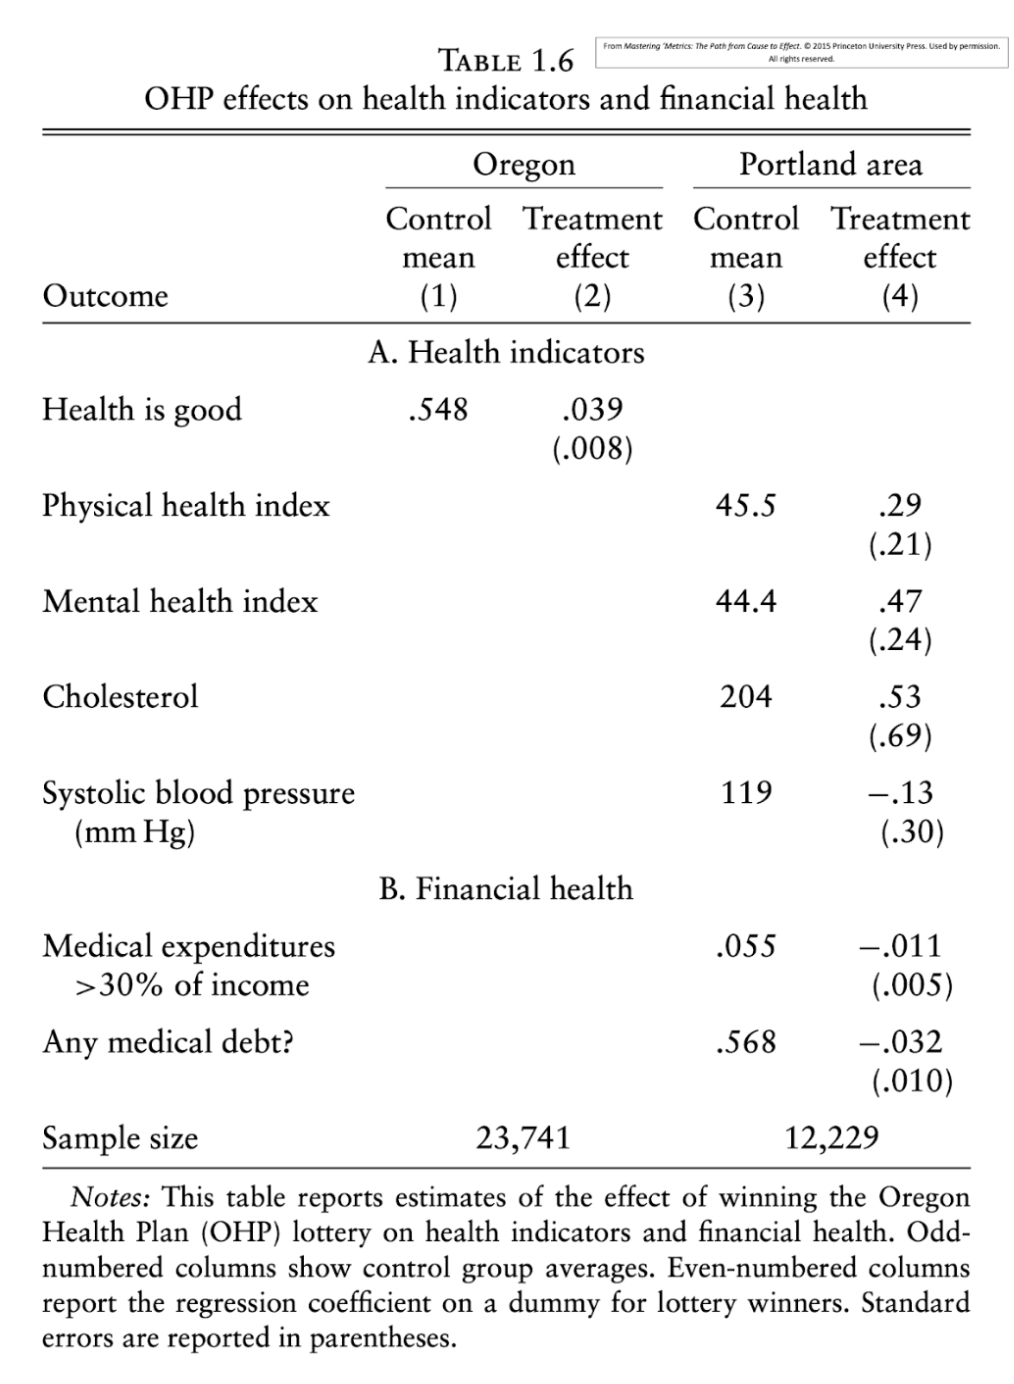
\includegraphics[width=3.3in]{Figures/midterm2_table1.png}
    %\caption{}
    \label{}
\end{figure}
 \begin{enumerate}
     \item How many regressions are in panel A of this table? 
    \begin{solution}
    Five (2pts). Seven (1pt) 
    \end{solution}
     \item Write down the regression equation for the Physical Health index (assume that the regression uses only the treatment variable as a regressor).
    \begin{solution}
    Physical Health index= 45.5 +0.29 * OHP treatment. 
    Given that the question did not explicitly said "regression estimate" the following solution is also fine:
    
    $Y_i = \alpha + \beta T_i + e_i$  With $Y_i$ Physical health index and $T_i$ OHP Treatement
    \end{solution}
     \item Is it statistically significant? Why?
     \begin{solution}
     $0.29/0.21<2$, not significant at 5\% level. 
     \end{solution}
 \end{enumerate}

 





\newpage
\item Recall this table from section 7 (“The gender gap in Canadian federal election…”) [8pts, 2pts each]: 

\centering
\begin{tabular}{lcc}
\hline \hline & (Model 1) & (Model 2) \\
\hline Woman & $-9.877^{* * *}$ & $-0.450^{* * *}$ \\
& $(0.366)$ & $(0.135)$ \\
Vote share lag & & $0.276^{* * *}$ \\
& & $(0.006)$ \\
Party performance & & $0.666^{* * *}$ \\
& & $(0.004)$ \\
Incumbent Party & & $6.783^{* * *}$ \\
& & $(0.148)$ \\
Distance from contention & & $-0.015^{* *}$ \\
& & $(0.005)$ \\
Constant & $27.682^{* * *}$ & $0.281$ \\
& $(0.139)$ & $(0.246)$ \\
\hline Observations $/ \mathrm{N}$ & 23903 & 23903 \\
$R^{2}$ & $0.030$ & $0.872$ \\
\hline \hline Standard errors in parentheses & & \\
${ }^{*} p<0.05,{ }^{* *} p<0.01,{ }^{* * *} p<0.001$ &
\end{tabular}

\raggedright
\begin{enumerate}[label=\alph*)]
    \item What is the corresponding equation for Model 2?, What is the estimated equation for Model 2?
    \begin{solution}
    Regression equation:
    \begin{equation*}
    \text{Outcome}_{i} = \alpha + \beta_{1}\times \text{Women}_{i} +\beta_{2} \times \text{Vote share lag}_{i} +\beta_{3} \times \text{Party performance}_{i} +\\ 
    \beta_{4} \times \text{Incumbent Party}_{i}+\beta_{5} \times \text{Distance from contention}_{i} +e_{i}
    \end{equation*}
    
   Full credit if the refer to the outcome in general terms (Y or outcome is fine)
   
   Estimated equation: 
   \begin{equation*}
         \centering
    \text{Outcome} = 0.281 -0.450\times \text{Women}+0.276 \times \text{Vote share lag}+0.666 \times \\\text{Party performance}+6.783 \times \text{Incumbent Party}-0.015 \times \text{Distance from contention}
    \end{equation*}
   
    \end{solution}
    \item Provide an interpretation of this coefficient using the idea of regression at matching.
     \begin{solution}
     
    On average women have -0.45 units less units (of the outcome) relative to men within \textbf{when comparing within groups (cells) of similar covariates/regressors (voter share, party performance, party incumbency, and distance from contention)}. Given that the question does not specify a specific variable, any variable is fine as long as it has the interpretation in bold (parenthesis is optional) 
    \end{solution}
    \item Provide an interpretation in plain English for the coefficient for the variable Women in model 2
     \begin{solution}
    Women have, on average, -0.45 of (outcome) when comparing individuals with similar characteristics (of voter share, party performance, incumbency and distance from contention)
    \end{solution}
    \item Compute the t-statistic, for standard the null of a zero coefficient, for the coefficient of the variable “Distance from contention” in model 2. Give a rough estimate of the corresponding p-value. 
    \begin{solution}
    $$t = \frac{-0.015-0}{0.005} =3 $$ (1pt) The p-value is smaller than 0.01 (1pt, with 0.5pt if they say smaller than 0.05).
    

    \end{solution}
  \end{enumerate}

 


\newpage
\item The regression residuals [2pts]
\begin{enumerate}[label=\alph*)]
 \item are aggregated in a sum to solve the regression minimization problem. 
 \item are unknown since we do not know the population regression function.
 \item are aggregated in a squared sum to solve the regression minimization problem. 
 \item should not be used in practice since they indicate that your regression does not run through all your observations.
  \end{enumerate}
\begin{solution}
C
\end{solution}
 
 \item Describe the OVB formula in one sentence (all English, no symbols) [3pts, 1 sentence]
\begin{solution}

Short equals long plus relationship between omitted and treatment times relationship between outcome and omitted in long (fine if instead of "relationship it say effect"). 
\end{solution}



\item In a video watched on lecture one, an interviewer brings up the point that the gender pay gap in the UK is 9\% as evidence that modern society is still primarily dominated by men. Her point is that gender causes a wage differential. \begin{enumerate}[label=\alph*)]
\item Write down the underlying regression that corresponds to interviewers' claim that women earn 9\% less than men on average in the UK?[2pts]
\begin{solution}
$$log(Wage) = \alpha -0.09 * Gender$$ 
where gender = 1 means women, =0 means men. 

-0.5 if outcome variable is not logged. 

Another possible solution : 
$$log(Wage) = \alpha + \beta * Gender$$ + e
With and estimated $beta= 0.09$. 

-0.5 if the answer puts estimated beta in the equation and the residual. 

\end{solution}

\noindent Let’s assume that another (new) commentator jumps into the conversation and says “That’s probably an underestimate once you take into account that women stay away from industries that have a bad record in the treatment of women, and that those industries tend to have lower earnings on average” 

\item Write down the underlying regression that corresponds to the new commentator’s argument (hint: think of an Industry Machismo Index (IMI), where 0 means no machismo in the industry and 100 means maximum machismo). [2pts]
\begin{solution}

$$log(Wage) = \alpha + \beta_{1} * Gender + \beta_{2} * IMI + e$$ 
The new commentator suggests there is OVB (but in a different direction than the previous commentator). If we control for IMI the gap would be larger ($\beta_{1}$ more negative) than the estimated coefficient of -0.09 from part (a).
\end{solution}


\item Discuss how the OVB formula could help us understand the effect of including a variable like “an industry machismo index” on the effect of gender on wages. Write down the long, short and auxiliary equations and interpret the OVB formula (the right hand side, not the $\beta_{l} -  \beta_{s}$ part) [3pts, 2-5 lines]
\begin{solution}

long: $log(Wage) = \alpha_{l} + \beta_{l} * Gender + \lambda* IMI + e_{l}$\\
short: $log(Wage) = \alpha_{s} + \beta_{s} * Gender + e_{s}$\\
auxiliary: 
$IMI = \pi_{0} + \pi_{1} * Gender +u$\\
$OVB= \beta_{s}-\beta_{l} = \lambda * \pi_{1}  $\\

"Women stay away from industries that have a bad record in the treatment of women" means $\pi_{1} <0$. "Those industries (with high IMI) tend to have lower earnings on average" means $\lambda <0$. As a result, $\beta_{s}-\beta_{l} >0$, so $\beta_{s}>\beta_{l}$ and since they are negative, the true effect ($\beta_{l}$) is even more negative (a larger gap). 
\end{solution}
 \end{enumerate}

\item High variation in \rule{1cm}{0.15mm}  increases the t-statistics regression coefficients (for 0 null hypothesis), while high variation in \rule{1cm}{0.15mm} reduces it.[3pts] 
\begin{enumerate}[label=\alph*)]
    \item the sample size; the residuals
    \item the residual; the sample size
    \item the regressor; the residual
    \item the residual; the regressor. 
\end{enumerate}
\begin{solution}
C
\end{solution}


(Table 4 is used in questions 18 and 19 below)

\begin{figure}[H]
    \centering
    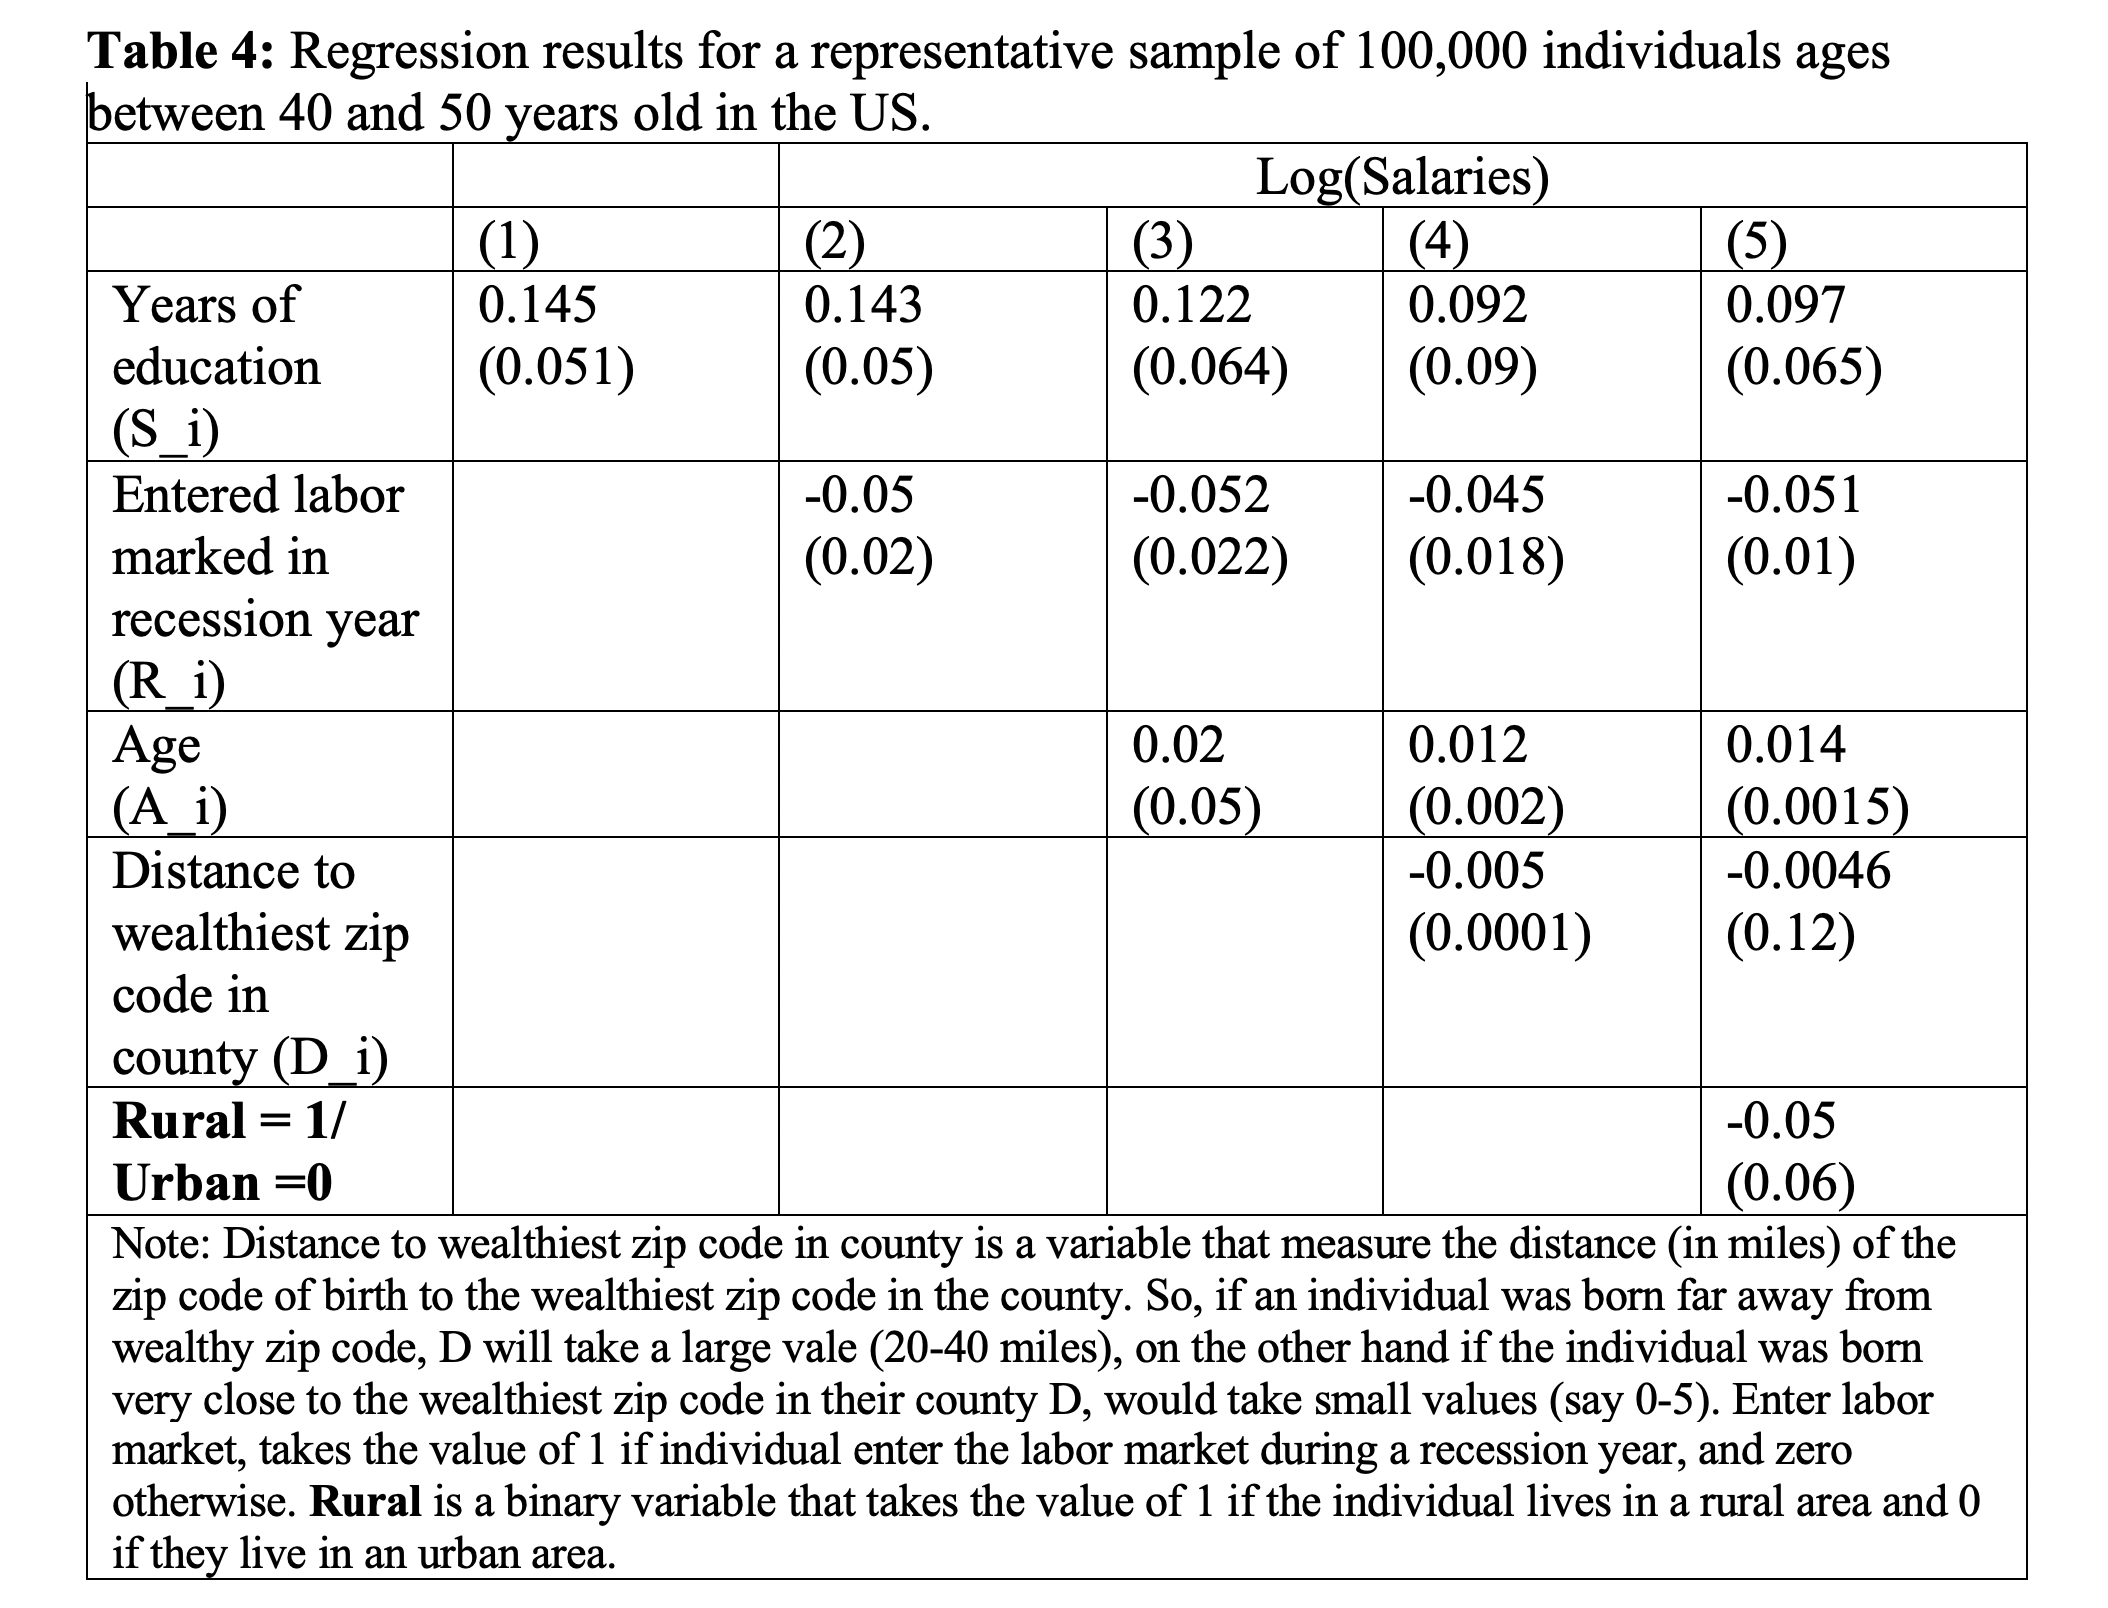
\includegraphics[width=5.3in]{Figures/midterm2_table4.png}
    %\caption*
    \label{}
\end{figure}

\item Based on OVB and Regression as Matching. Answer the following questions related to Table 4: [12pts]
\begin{enumerate}[label=\alph*)]
    \item Interpret the coefficient for years of education in the \textbf{second} column using the idea of regression as matching. [3pts]
    \begin{solution}
    One additional year of education is associated with a 14.3\% increase in salary when comparing individuals that enter the labor force in similar recession years (or years of economics activity, or something similar). 
    \end{solution}

    \item Write down the regression equation for \textbf{column (3)}[2pts]
    \begin{solution}
    $$log(Salaries) = \alpha + \beta_1 S_{i} + \beta_2 R_{i} + \beta_3 Age_{i} + e_$$
    \end{solution}
    
-0.5pts If the answer focuses on the estimated regression equation (-0.5pt additional if the answer includes the residual in the estimated regression)

    \begin{solution}
    $$log(Salaries) = \alpha + 0.122 S_{i} -0.052 R_{i} +0.02 Age_{i}$$
    \end{solution}
    
    \item Using the OVB formula, explain what is going on with the coefficient on years of education, when we move from 1 to 2, and from 3 to 4. Be explicit about the auxiliary equation that you would need in each case.  (Note: by OVB formula, we mean the right-hand side, not “beta long – beta short) [3pts, 2-4 lines]
     \begin{solution}
  \textbf{  From 1 to 2:}\\
long: $Log(Salaries) = \alpha_{l 1} + \beta_{l 1} \times S_{i} + \lambda_{1}* R_{i} + e_{l 1}$\\
short: $Log(Salaries) = \alpha_{s 1} + \beta_{s 1} \times S_{i} + e_{s 1}$\\
auxiliary: 
$R_{i} = \pi_{0} + \pi_{1} \times S_{i} +u_{1}$\\
$OVB= \beta_{s 1}-\beta_{l 1} = \lambda_{1} * \pi_{1} =0.145 - 0.143 = -.002$\\
The lack of substantial OVB is due to no relationship between entering in a recession and years of education ($\pi_{1}$ close to 0).  

   \textbf{ From 3 to 4:} \\
    long: $Log(Salaries) = \alpha_{l 2} + \beta_{l 2} \times S_{i} + \beta_{l 3}  \times R_{i} + \beta_{l 4}  \times A_{i} + \lambda_{2}  \times D_{i} + e_{l 2}$\\
short: $Log(Salaries) = \alpha_{s 2} + \beta_{s 2} \times S_{i} + \beta_{s 3}  \times R_{i} + \beta_{s 4}  \times A_{i} + e_{s 2}$\\
auxiliary: 
$D_{i} = \pi_{2} + \pi_{3} \times A_{i} +u_{2}$\\
$OVB= \beta_{s 2}-\beta_{l 2} = \lambda_{2} * \pi_{3} =0.122 - 0.092 = 0.03 > 0 $\\
The presence of substantial bias reflects implies that there must be a significant (negative) relationship between education and distance to wealthy areas ($\pi_{3}<0$). 
     \end{solution}
     
    \item In order to capture the true causal effect, it would be helpful to have some measure of “ability” (think something like general score of “skills and talents”) and of “privilege” (think something like a general score for additional support received during upbringing and in labor market) both unobservable. Using the OVB formula (again, not the difference between beta long and beta short, but the other side of the equation), argue about the sign of the bias each of this two unobservable will generate. [4pts, 2-5 lines]
\end{enumerate}
    For simplicity lets use the columns 1 as the short equation (answer is fine if it uses any column as short): 
    \begin{solution}
    
    \begin{align*}
    \text{Short: } &\quad Y_i = \alpha^{s} + \beta^{s} S_{i} +  e^{s}_{i}\\
    \text{Long Ability: }  &\quad Y_i = \alpha^{s} + \beta^{s} S_{i} + \gamma Ability_i +  e^{l}_{i}\\
    \text{Long Privilege: }  &\quad Y_i = \alpha^{s} + \beta^{s} S_{i} + \lambda Privilege_i + e^{l}_{i}\\
    \text{Aux Ability: }  &\quad Ability_i = \pi_{a,0} + \pi_{a,1} S_{i} + e^{a}_{i}\\
    \text{Aux Privilege: }  &\quad Privilege_i = \pi_{p,0} + \pi_{p,1} S_{i} + e^{p}_{i}
    \end{align*}
    (optional: Assuming higher ability, and higher privilege are capture by a higher score) The traditional story is that more ability correlates positively with both income and schooling. Similarly more privilege correlates positively with both income and schooling. Hence,  OVB tells us that. 
     \begin{align*}
    OVB_{Ability} &= \pi_{a,1} \gamma > 0\\
    OVB_{Privilege} &=   \pi_{p,1} \lambda > 0
    \end{align*}   
    \end{solution}

\item Based on All Things Regression (Anatomy and others): Answer the following questions related to Table 4: [8pts] 
\begin{enumerate}[label=\alph*)]
\item Write down the two-regressions required to generate the coefficient of \textbf{distance to wealthiest zip code} in column 5 as the coefficient of a bi-variate regression equation. [2pts]

\begin{solution}

    \begin{align*}
     Y_i &= \alpha + \beta_4 \widetilde D_{i} +  e^_{i}\\
     D_{i} &= \pi_0 + \pi_1 S_{i} + \pi_2 R_{i} + \pi_3 A_{i} + \pi_4 Rural_i + \widetilde D_{i} 
    \end{align*}

\end{solution}

\item What is the t-statistic, for a null of zero association, for the coefficient on distance to wealthiest zip code on columns (4) and (5)? What happened with the coefficient themselves?  Can you think of a possible explanation (hint: think of regression [2pts] anatomy)? [4pts]

\begin{solution}
t-statistics for columns 4 and 5 are -50 and about 0.04 (enough if the answer says much smaller than 2). The coefficient did not change substantially (2pts). This happens when the new variable included (Rural) is highly collinear with the one that dropped in significance (the formula for the SE using regression anatomy shows that lower variation in the residualized regressor makes the regressors increase drastically). 


\end{solution}

\item Assume that the person that gives you the regression outputs tells you “I forgot to mentioned that the variable for years of education was actually in logs”, how should you re-interpret this coefficient? [2pts]

\begin{solution}
In this case the coefficient becomes an elasticity (or in what percent Y changes when S changes 1 percent). Hence the interpretation would be that salary increases in 0.13\% when education increases in 1\%.  
\end{solution}
\end{enumerate}
 \vspace{2cm}
 
 \clearpage


\end{enumerate}
\end{document}